\documentclass[a4paper,titlepage,french]{report}
\usepackage[T1]{fontenc}
\usepackage[french]{babel}
\usepackage[utf8x]{inputenc}
\usepackage{amsmath}
\usepackage{eurosym}
\usepackage{float}
\usepackage{graphicx}
\usepackage[colorinlistoftodos]{todonotes}
\usepackage{placeins}
\usepackage{verbatim}
\usepackage{fmtcount}
\usepackage{array}
\usepackage{url}
\usepackage[toc,page]{appendix} 
\renewcommand{\arraystretch}{1.25}

\usepackage{tabularx}
\newcounter{cptspec}
\setcounter{cptspec}{0}
 
\title{INSA de Rennes \\ Quatrième année Informatique \\ \bigskip \hrule \bigskip Rapport de conception \\ \bigskip Projet Value-at-Risk \bigskip \hrule}

\author{Benjamin \bsc{Bouguet} - Damien \bsc{Carduner} \\Paul \bsc{Chaignon} - Eric \bsc{Chauty} - Xavier \bsc{Fraboulet} \\ Clément \bsc{Gautrais} - Ulysse \bsc{Goarant} \\ ~~\\
Hamdi \bsc{Raissi} - Ivan \bsc{Le Plumey} \\ Quentin \bsc{Giai Gianetto}}


\date{Janvier 2014}

\begin{document}
\maketitle

\thispagestyle{empty}
\newpage

~~
\thispagestyle{empty}
\newpage

% TODO Add Introduction to the table.
\tableofcontents
\newpage

\listoffigures
\newpage

% TODO Change portefolio to portfolio in diagrams.
% TODO Classes and sequence diagrams are not coherent.
% TODO Justify a bit more the use of all patterns.
% TODO Explain in a line the patterns.
% TODO Check number of hours for report generations in GANTT.


\addcontentsline{toc}{chapter}{Introduction}
\chapter*{Introduction}

Dans les salles de marchés, les traders achètent et vendent des actions et obligations, pour le compte de grandes banques ou investisseurs toujours à la recherche d'un maximum de profits pour des pertes minimales.
% TODO Hamdi: Mal dit : il s'agit plus de quantifier les risques de pertes pour prévoir des montants adéquats pour couvrir les pertes éventuelles.
Les financiers sont intéressés par le montant maximal qu'ils peuvent perdre pour un portefeuille d'actifs donné.
En connaissant ce montant, leurs prévisions n'en seront que plus fiables et permettront peut-être d'éviter de mauvais placements.

C'est précisément ce que notre logiciel permettra de faire : calculer la Value-at-Risk par diverses méthodes statistiques.
Néanmoins, un unique calcul de la Value-at-Risk n'est pas suffisant pour permettre de bonnes prévisions.
Pour cette raison, notre programme aura l'avantage de proposer un ensemble de tests, comparaisons, tableaux récapitulatifs et même de la comparaison de méthodes statistiques par backtesting.
Avec cette multitude d'outils, les financiers seront en mesure de travailler sur leurs portefeuilles aisément, au moyen d'outils de manipulations des actifs, mais aussi d'une interface intuitive et ergonomique, pensée pour ne montrer que l'essentiel et être facile d'utilisation.

Le rapport de spécifications fonctionnelles détaillait de manière très précise nos choix d'implémentation pour ce projet.
Nous devons maintenant détailler nos choix techniques ainsi que nos décisions de modélisation.
Dans un premier temps, nous allons rappeler les principales fonctionnalités de notre logiciel.
Puis nous décrirons l'architecture globale du logiciel ainsi que les interactions entre les différents modules.

Dans un deuxième temps, nous décrirons à partir de diagrammes de classes et de séquences nos différents choix de conception.
\`A partir desquels, nous détaillerons nos choix d'implémentations et d'interfaçage.


\chapter{Rappel des spécifications}

\section{Cas d'utilisations}

L'utilisateur de notre application aura besoin d'un ensemble d'outils pour gérer comme il le souhaite ses portefeuilles, effectuer des calculs et prendre ses décisions. Ceci peut se diviser en 3 grands pôles :
\begin{itemize}
\item la gestion de portefeuille;
\item le calcul de la Value-at-Risk;
\item le backtesting.
\end{itemize}
 
Ces derniers ont des dépendances respectives diverses. Par exemple, le backtesting utilise des fonctions du second pôle.
En effet, son but est de comparer les différentes méthodes de calcul de la Value-at-Risk.
Ces deux derniers modules devront stocker des résultats dans le portefeuille associé.
Ces différentes interactions sont bien visibles à la figure \ref{fig:usecase}.

\begin{figure}[h]
 	\center
  	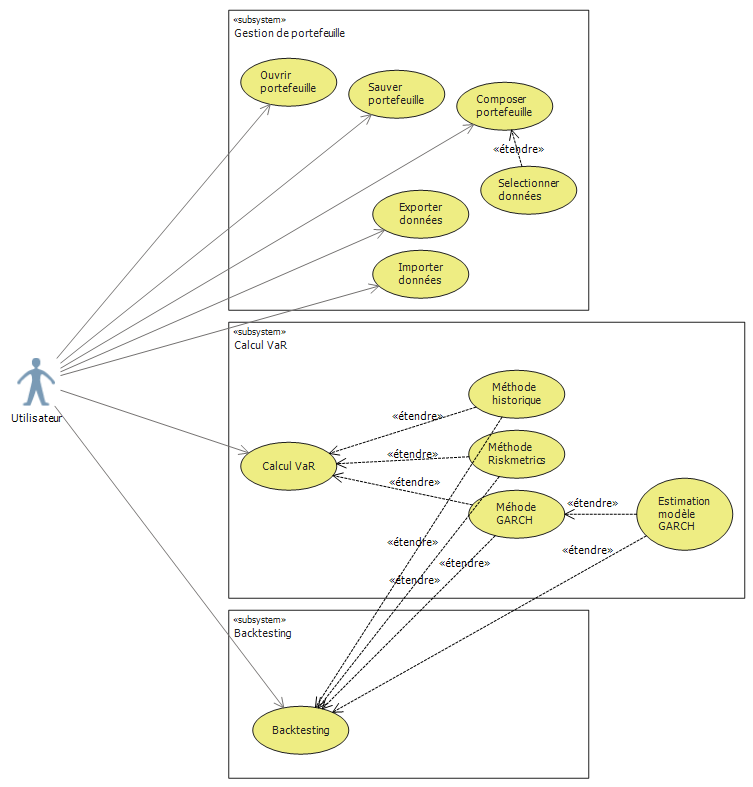
\includegraphics[scale=0.8]{UseCaseConception.png}
  	\caption{Diagramme des cas d'utilisation}
	\label{fig:usecase}
\end{figure}

Ces trois grands pôles sont détaillés dans les parties suivantes.


\section{Gestion de portefeuille}

La première étape dans toute gestion de portefeuille est la création.
Pour cela, il faut commencer par importer des actifs stockés dans des fichiers de type CSV comme ceux fournis par Yahoo Finance par exemple.
Ensuite l'utilisateur pourra sélectionner les données qu'il souhaite pour les ajouter dans un nouveau portefeuille. Il affectera alors une pondération (nombre d'actions de cet actif).
Par exemple, la figure \ref{fig:csvexample} correspond au contenu d'un actif au format CSV provenant de Yahoo Finance.
Nous utiliserons seulement les colonnes \textit{Date} et \textit{Close}.

\begin{figure}[h]
  \center
    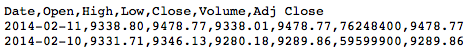
\includegraphics[scale=0.5]{yahoo-dax-csv-example.png}
    \caption{Extrait d'un actif au format CSV}
  \label{fig:csvexample}
\end{figure}

\section{Calcul de la Value-at-Risk}

Le calcul de la Value-at-Risk est la fonctionnalité centrale de ce logiciel. Comme dit précédemment, elle s'effectue sur un portefeuille donné.
De plus, le calcul de la Value-at-Risk se caractérise par la méthode utilisée (historique, Riskmetrics ou selon un modèle GARCH), un niveau de risque et un horizon de temps.
Il sera donc possible de calculer la Value-at-Risk selon les différentes méthodes et selon les paramètres précédemment décrits sur chacun des portefeuilles créés.
Les résultats seront alors affichés dans un rapport. Néanmoins, proposer un simple calcul de Value-at-Risk n'est pas suffisant pour permettre une prise de décision.
Il faut aussi s'assurer que le calcul est fiable.
Pour cela, l'utilisateur pourra effectuer du backtesting.


\section{Backtesting}

Le backtesting permet d'évaluer et de comparer les différentes méthodes de calcul de la Value-at-Risk.
L'ensemble des résultats générés seront disponibles dans un rapport associé au portefeuille.

Lorsque l'utilisateur souhaite faire du backtesting, il doit choisir le portefeuille sur lequel l'effectuer, la ou les méthodes de calcul de la Value-at-Risk (historique, Riskmetrics ou GARCH), la période de test, le risque et l'horizon de temps.


\section{Diagramme de composants}

La figure \ref{fig:diagramme-composants} présente le diagramme des composants internes de notre logiciel.
Nous avons réalisé les diagrammes de classes des différents composants séparément dans un premier temps.
Les diagrammes de séquences nous ont ensuite permis d'établir les liens entre nos divers composants.

% TODO Redo the composants diagram.

\begin{figure}
  	\center
  	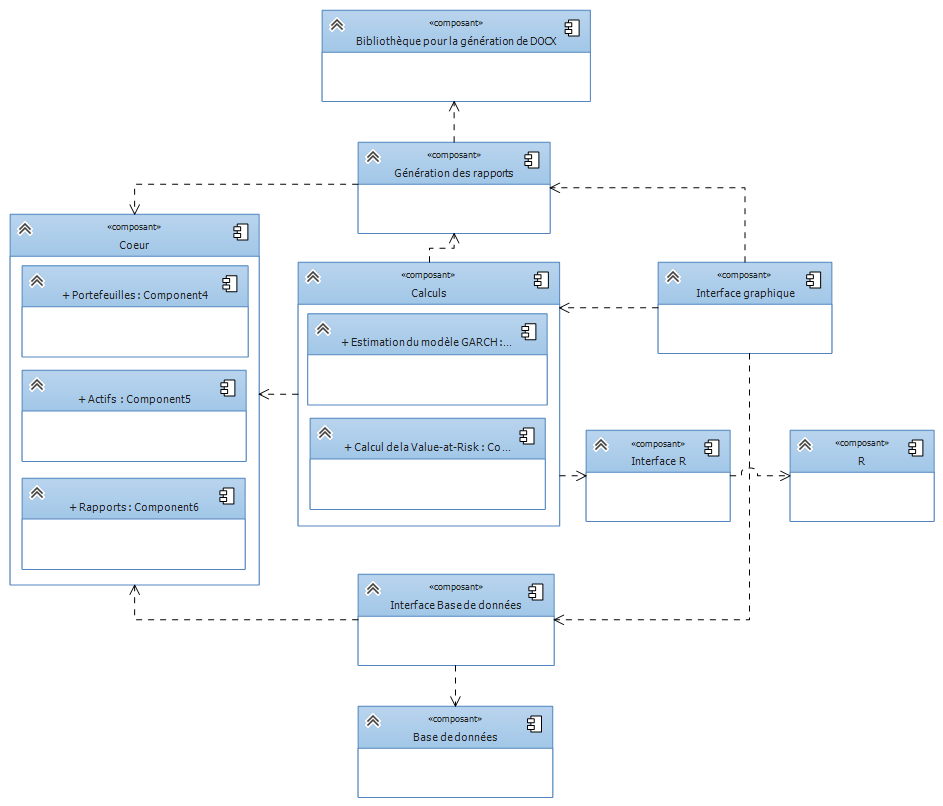
\includegraphics[width=1\textwidth]{architecture_generale.png}
  	\caption{Diagramme des composants internes}
  	\label{fig:diagramme-composants}
\end{figure}



\chapter{Conception}

\section{Modélisation de la base de données}

\subsection{Modélisation}

La modélisation des données est organisée autour des portefeuilles.
Un portefeuille est composé d'un nombre variable d'actifs avec diverses pondérations.
Tous les rapports sont associés à un portefeuille.

De plus, un portefeuille sera amené à évoluer.
Des actifs pourront par exemple être ajoutés, constituant ainsi un nouveau portefeuille dérivant du premier.
Comme nous souhaitons conserver l'historique de ces évolutions nous garderons une référence vers le portefeuille d'origine dans le nouveau portefeuille.

Enfin, les valeurs des actifs seront conservées dans les fichiers CSV et XSL importés. 
La base de données contiendra donc des références vers ces fichiers.
L'entité \textit{Actifs} contient aussi l'intervalle de temps sur lequel est défini un actif.
De même que pour les actifs, l'entité \textit{Rapports} contiendra uniquement des références vers les fichiers générés.

La figure \ref{fig:modele-entite-association} présente le modèle entité-association de notre base de données.
Nous en déduisons directement ses tables dans la figure \ref{fig:base-donnees}.
Il apparaît clairement que l'unique association ne pouvant être intégrée dans une entité est \textit{Composé de}.
Cette dernière constituera donc la table Pondérations pour faire le lien entre les portefeuilles et les actifs les constituant.
Le champ \textit{parent} de \textit{Portefeuilles} sera nul pour représenter l'absence de parent.

\begin{figure}
  	\center
  	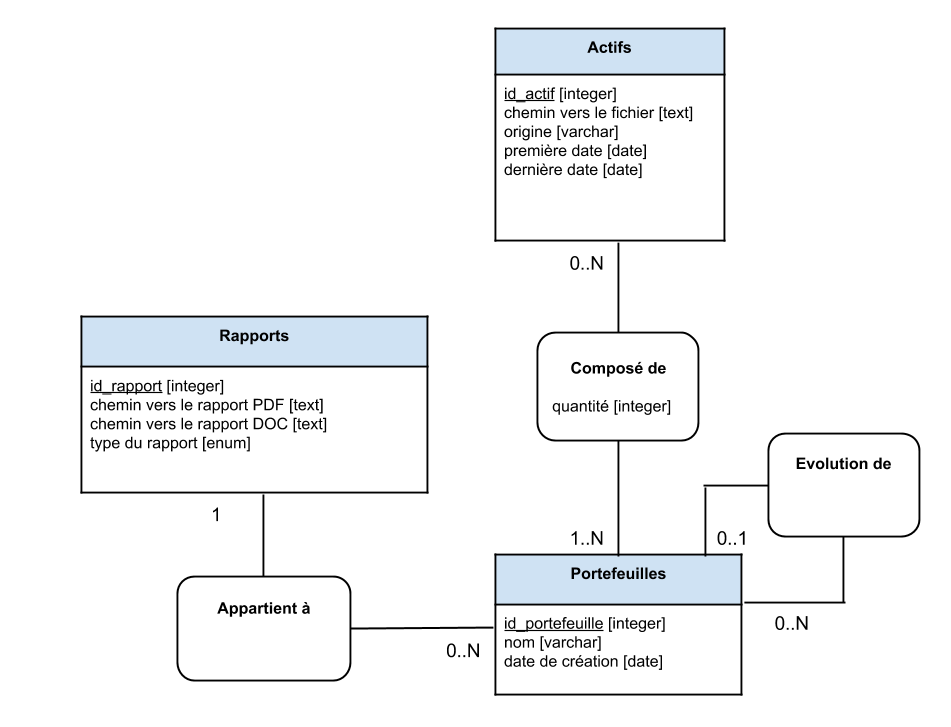
\includegraphics[width=1\textwidth]{modele-entite-association.png}
  	\caption{Modèle entité-association}
  	\label{fig:modele-entite-association}
\end{figure}

\begin{figure}
  	\center
  	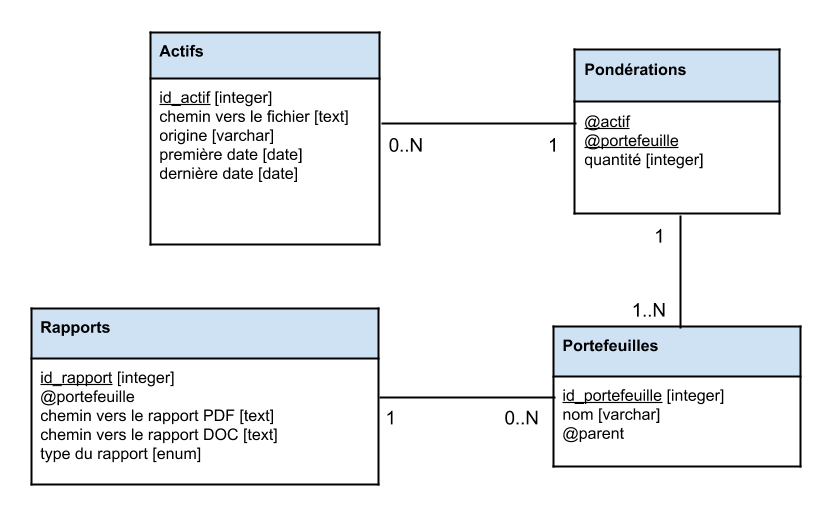
\includegraphics[width=1\textwidth]{base-donnees.png}
  	\caption{Base de données}
  	\label{fig:base-donnees}
\end{figure}


\subsection{Choix du Système de Gestion de Base de Données}

Le nombre d'informations sauvegardées dans la base de données restera toujours raisonnable.
La table dont la taille sera la plus importante sera vraisemblablement \textit{Actifs}.
Cependant le nombre d'actifs devraient rarement dépasser le millier.
De plus, nous n'avons pas besoin de gérer d'accès concurrentiels à la base de données.

Nous pouvons donc utiliser le SGBD SQLite qui a l'avantage de ne pas nécessiter de serveur \cite{website:SQLite}.
De plus, toute la base de données sera contenue dans un unique fichier et les accès en lecture comme en écriture seront beaucoup plus rapides qu'avec un SGBD traditionnel.


\section{Diagrammes de classes}

Cette partie détaille la modélisation pour les différents composants de notre logiciel.
Nous commençons par la modélisation des données de base. Nous abordons ensuite le problème de l'instanciation des actifs.
La suite des modélisations expliquent les composants nécessaires à la génération des rapports en passant par les interfaces avec quelques modules externes.
Enfin, nous finissons avec le chargement de session et la fonctionnalité d'importation/exportation de portefeuilles.


\subsection{Modélisation des portefeuilles}

La modélisation sous forme de classes des données en figure \ref{fig:diagramme-classes-donnees} est analogue à celle pour la base de données. Un portefeuille contient des références vers ses rapports et ses actifs. Les divers attributs présents dans la base de données sont aussi présents ici.

De plus, un portefeuille dispose de deux méthodes pour calculer son intervalle de définition à partir de ceux de ses actifs.

% TODO Change name of getFirstDate...
\begin{figure}
  	\center
  	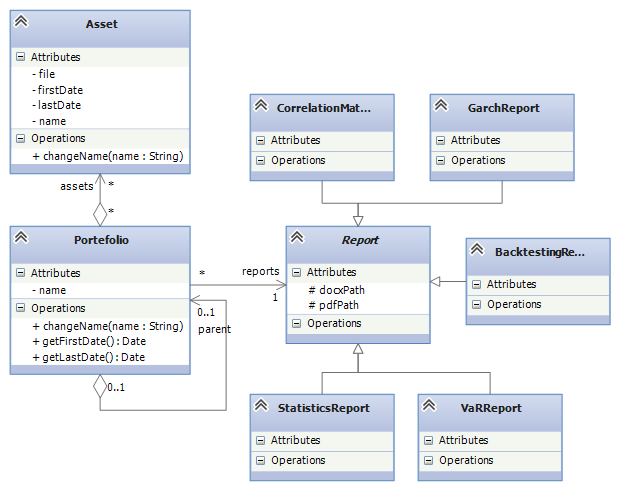
\includegraphics[width=1\textwidth]{diagramme-classes-donnees.png}
  	\caption{Diagramme de classes des données}
  	\label{fig:diagramme-classes-donnees}
\end{figure}


\subsection{Instanciation des actifs}

Un même actif peut participer à la constitution de plusieurs portefeuilles.
Il pourra donc être référencé dans plusieurs objets.
Pour éviter toute duplication nous utiliserons un patron de conception \textit{Poids-Mouche} présenté en figure \ref{fig:diagramme-classes-flyweight}.
Nous aurons donc une \textit{Fabrique} d'actifs qui conservera une référence vers tous les actifs instanciés. Cette dernière est aussi un \textit{Singleton}.

\begin{figure}
  	\center
  	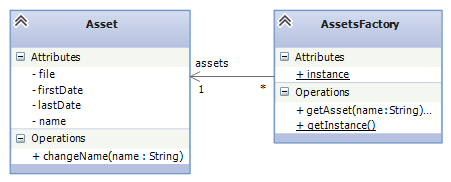
\includegraphics[width=1\textwidth]{diagramme-classes-flyweight.png}
  	\caption{Diagramme de classes \textit{Poids-mouche} pour l'instanciation des actifs}
  	\label{fig:diagramme-classes-flyweight}
\end{figure}


\subsection{Calcul de la Value-at-Risk}

Notre logiciel proposera trois méthodes\footnote{La méthode historique, la méthode Riskmetrics et la méthode avec modélisation GARCH} différentes pour calculer la Value-at-Risk.
Nous utiliserons un patron de conception \textit{Stratégie} (présenté en figure \ref{fig:diagramme-classes-var-strategy}) pour modéliser ces méthodes.

Les trois stratégies prennent en entrée un portefeuille, un niveau de risque et un horizon de temps.
Cependant, la méthode avec modélisation GARCH prend aussi en entrée le modèle GARCH.
En effet, nous avons choisi d'externaliser l'estimation du modèle GARCH pour faciliter d'autres opérations (voir Backtesting avec modèle GARCH en \ref{backtesting-modele-garch}).
La stratégie avec modélisation GARCH pourra donc être instanciée avec différents modèles GARCH.

Toutes les stratégies seront instanciées pour un certain portefeuille et un certain niveau de risque.
L'horizon de temps sera quant à lui passé en argument de la méthode de calcul, toujours pour faciliter le backtesting.

\begin{figure}
  	\center
  	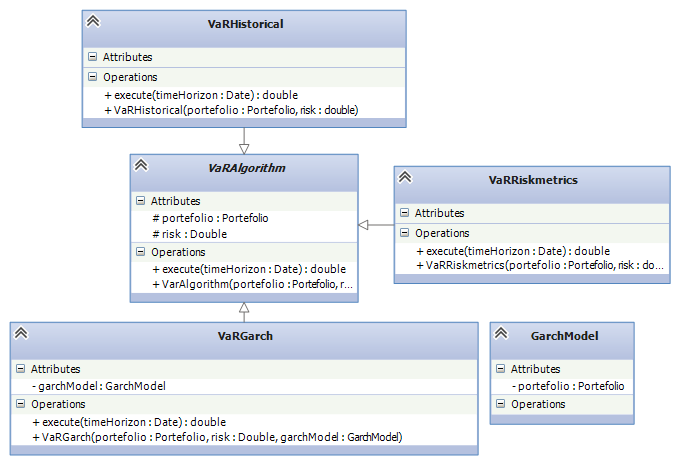
\includegraphics[width=1\textwidth]{diagramme-classes-var-strategy.png}
  	\caption{Diagramme de classes \textit{Stratégie} pour le calcul de la Value-at-Risk}
  	\label{fig:diagramme-classes-var-strategy}
\end{figure}


\subsection{Génération des rapports}

Les rapports seront générés aux formats PDF et DOCX.
L'opération pourra donc prendre un peu de temps.
Cette génération sera effectuée par une classe \textit{ReportsFactory}.

Les différents types de rapports nécessitent des informations différentes pour leur génération.
Nous utiliserons donc le patron de conception \textit{Fabrique} présenté en figure \ref{fig:diagramme-classes-reports-factory}.
Les informations pour la génération seront passées à la fabrique lors de son instanciation.

\begin{figure}
  	\center
  	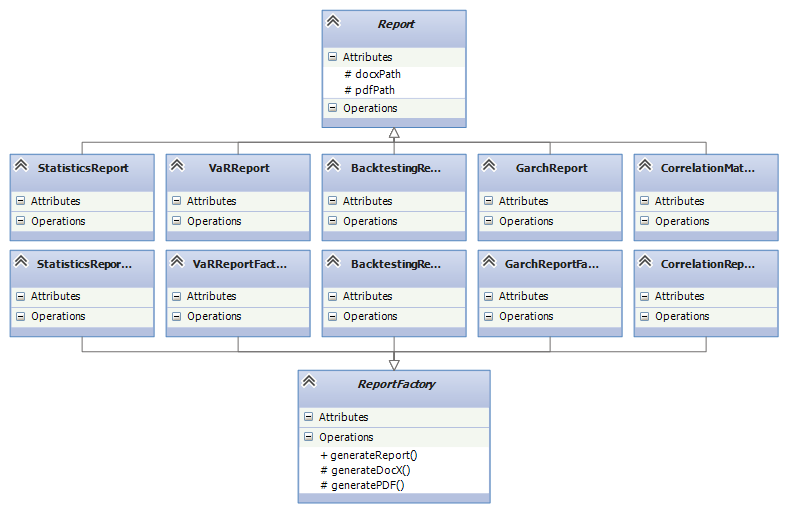
\includegraphics[width=1\textwidth]{diagramme-classes-reports-factory.png}
  	\caption{Diagramme de classes pour la création des classes \textit{Report}}
  	\label{fig:diagramme-classes-reports-factory}
\end{figure}


\subsection{Composants externes}

Notre logiciel utilisera des composants externes pour répondre à certains besoins.
Nous utiliserons la bibliothèque SQLite pour la base de données, des scripts R pour les calculs statistiques complexes et deux bibliothèques pour la génération des rapports.

\subsubsection{Interface avec la base de données}

Notre session sera conservée dans une base de données SQLite.
Nous aurons quatre situations d'accès au fichier SQLite :

\begin{itemize}
	\item La sauvegarde de la session courante \footnote{La sauvegarde sera une action déclenchée par l'utilisateur uniquement.}.
  	\item L'ouverture d'une session.
  	\item Nous aurons aussi besoin d'accéder à la base de données lors de l'ajout d'un actif.
	Une méthode \textit{saveAsset} permettra alors de sauvegarder ce dernier.
  	\item Enfin, lors de son premier appel \footnote{\textit{AssetsFactory.getInstance} sera appelé pour la première fois lors de la construction de la session par \textit{SessionBuilder.buildSession}.}, le \textit{Singleton} \textit{AssetsFactory} chargera l'ensemble des actifs à l'aide de \textit{buildAssets}.
	Si de nouveaux actifs sont créés par la suite \textit{AssetsFactory} les chargera uniquement lorsqu'un portefeuille en aura besoin à l'aide de la méthode \textit{buildAsset}.
\end{itemize}

La figure \ref{fig:diagramme-classes-interface-bdd} présente les deux classes de sauvegarde et de restauration des sessions. Ces deux classes hériteront d'une classe \textit{SQLiteManager} mettant à disposition des méthodes générales d'accès à la base de données.

\begin{figure}
  	\center
  	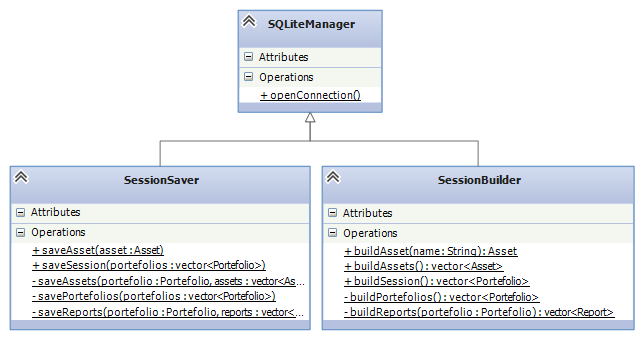
\includegraphics[width=1\textwidth]{diagramme-classes-interface-bdd.png}
  	\caption{Diagramme de classes pour la gestion de la session}
  	\label{fig:diagramme-classes-interface-bdd}
\end{figure}


\subsubsection{Appel des scripts R}

Certains calculs seront réalisés par des scripts R \cite{website:R}.
En effet ce langage est très bien adapté pour les calculs statistiques.
\`A cet effet nous utiliserons la classe utilitaire décrite en figure \ref{fig:diagramme-classes-interface-r}.
Elle permettra d'estimer le modèle GARCH et d'effectuer les tests de corrélation.

Les appels aux scripts R seront effectués en utilisant la bibliothèque \textit{RInside} \cite{website:RInside}. Cette dernière est bien documentée et permet simplement d'exécuter du code R dans du code C++.

\begin{figure}
  	\center
  	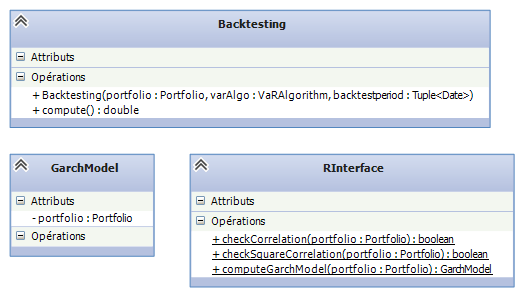
\includegraphics[width=1\textwidth]{diagramme-classes-interface-r.png}
  	\caption{Diagramme de classes interfaces avec R}
  	\label{fig:diagramme-classes-interface-r}
\end{figure}


\subsubsection{Génération des rapports}
%TODO vérifier la possibilité de conversion DOCX PDF

Pour la génération des rapports PDF et DOCX, nous nous appuierons sur des bibliothèques externes (libopc \cite{website:libopc} pour les DOCX et libHaru \cite{website:libHaru} pour les PDF).
Nous n'utiliserons qu'un petit ensemble des possibilités offertes par ces bibliothèques pour réaliser des opérations très similaires pour tous les types de rapports.

Pour cette raison la manipulation de ces bibliothèques sera réalisée par deux classes permettant d'effectuer les opérations nécessaires.
Nous aurons, par exemple, besoin d'une méthode \textit{addChart} pour ajouter un graphique dans un rapport et cela quel que soit le type du rapport.

Ces deux classes sont présentés à la figure \ref{fig:diagramme-classes-interface-report}.
Cette organisation est celle d'un patron de conception \textit{Monteur} où les appels des méthodes de construction sont effectués par les classes héritant de \textit{ReportFactory}.

\begin{figure}
  	\center
  	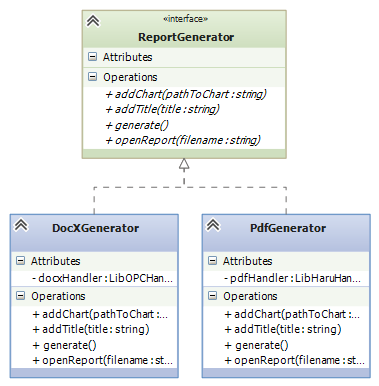
\includegraphics[width=0.7\textwidth]{diagramme-classes-interface-report.png}
  	\caption{Diagramme de classes interfaces avec les bibliothèques pour la génération des rapports}
  	\label{fig:diagramme-classes-interface-report}
\end{figure}


%\subsubsection{Génération des graphiques}

Nous génèrerons les graphiques intégrées aux rapports à l'aide QCustomPlot.
La création de graphiques est aussi possible avec R mais QCustomPlot nous permettra une plus grande maîtrise leur aspect.
QCustomPlot est habituellement utilisé pour afficher les graphiques créés.
Nous nous contenterons de les sauvegarder sous forme de fichiers sans les afficher.
Ainsi, ils pourront être utilisés lors de la compilation des rapports.


\subsection{Chargement de la session}

\`A l'ouverture de la session, tous les objets nécessaires seront chargés en mémoire vive depuis la base de données.
Nous devrons donc instancier les objets portefeuilles, rapports et actifs.
Nous utiliserons pour cela le patron de conception \textit{Monteur} décrit au niveau de la classe \textit{SessionBuilder} de la figure \ref{fig:diagramme-classes-interface-bdd}.


\subsection{Importation et exportation de portefeuilles}

Les fonctionnalités d'importation et d'exportation doivent permettre à un utilisateur d'exporter un ou plusieurs portefeuilles de sa session courante pour les importer dans une autre session.
L'importation doit pouvoir être réalisée sur un autre ordinateur disposant du logiciel.
De plus, l'utilisateur n'a pas besoin d'être capable de modifier le fichier d'export sans utiliser le logiciel.

Nous utiliserons pour cela un processus de sérialisation vers un fichier binaire.
L'utilisateur pourra choisir d'exporter les rapports associés à un portefeuille ou seulement le portefeuille lui-même.
Les actifs composant un portefeuille seront nécessairement exportés avec ce dernier.
Nous aurons donc divers types d'objets à sérialiser.
Tous ces objets disposeront de deux méthodes pour la sérialisation et la désérialisation.
Nous utiliserons la classe \textit{QVariant} de Qt à cet effet.


\section{\'Etudes de cas}

\subsection{Création d'un portefeuille}
Un portefeuille peut être créé à partir de zéro ou en modifiant un autre portefeuille.
Dans les deux cas l'utilisateur doit choisir les actifs à ajouter (et/ou à supprimer dans le second cas).

La figure \ref{fig:diagramme-sequence-creation-portefeuille} présente le diagramme de séquence de cette création.
% TODO Add a few comments on the conclusion from this diagram maybe?

\begin{figure}
  	\center
  	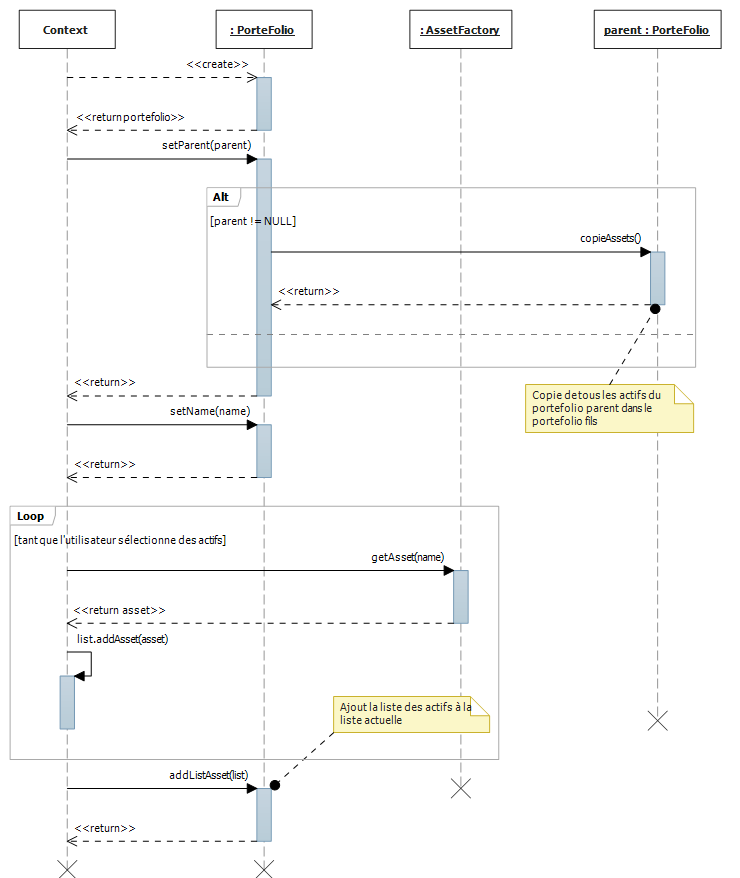
\includegraphics[width=1\textwidth]{diagSeqPortfolio.png}
  	\caption{Diagramme de séquence de la création d'un portefeuille}
    \label{fig:diagramme-sequence-creation-portefeuille}
\end{figure}


\subsection{Calcul de la Value-at-Risk avec modèle GARCH}

Le calcul de la Value-at-Risk avec un modèle GARCH nécessite dans un premier temps l'élaboration du modèle en lui-même.
Ce dernier s'obtient par la méthode \textit{getGarchModel} qui prend le portefeuille en paramètre.
Cette modélisation est ensuite utilisée par la classe \textit{VaRGarch} pour effectuer le calcul de la Value-at-Risk.
La figure \ref{fig:diagramme-sequence-var-garch} détaille ces opérations.

\begin{figure}
  	\center
  	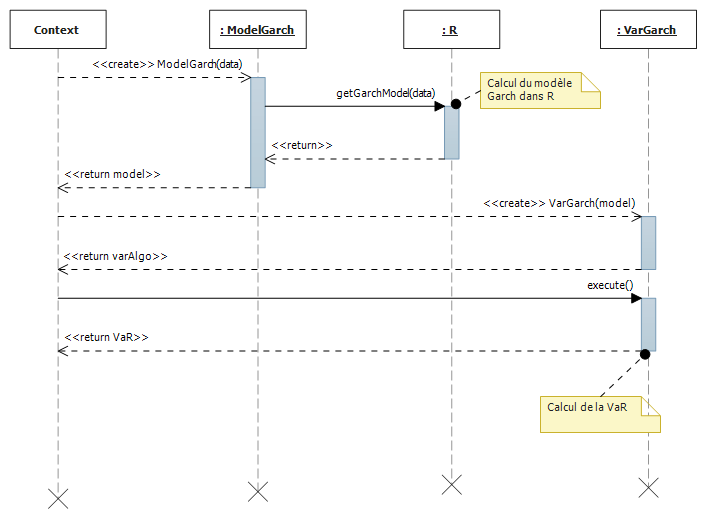
\includegraphics[width=1\textwidth]{diagSeqGarch.png}
  	\caption{Diagramme de séquence du calcul de la Value-at-Risk par GARCH}
    \label{fig:diagramme-sequence-var-garch}
\end{figure}


\subsection{Backtesting avec modèle GARCH}
\label{backtesting-modele-garch}

Un objet \textit{Backtesting} est instancié avec les attributs suivants : la classe de calcul de la Value-at-Risk, le portefeuille, la période de temps sur laquelle les tests doivent s'effectuer, le risque associé à la Value-at-Risk et son horizon de temps.
Cet objet possède une méthode \textit{backtest} qui effectue le backtesting.
Cette méthode fait un appel itératif au calcul de la Value-at-Risk selon la méthode correspondante sur chacun des jours de la période fixée.
La figure \ref{fig:diagramme-sequence-backtesting-garch} détaille ces opérations.

\begin{figure}
	\center
	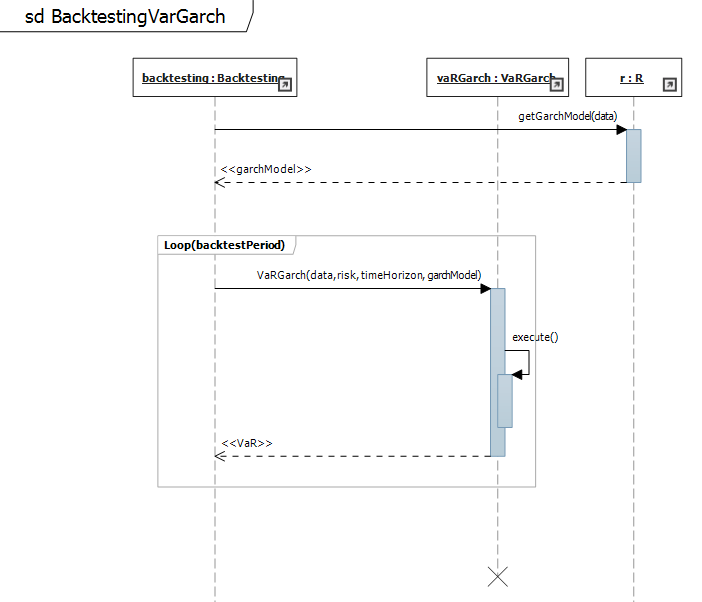
\includegraphics[scale=0.8]{diagramme_sequence_backtesting.png}
    \caption{Diagramme de séquence du Backtesting avec méthode GARCH}
    \label{fig:diagramme-sequence-backtesting-garch}
\end{figure}


\section{Interface graphique}

Nous avons décidé d'utiliser l'architecture Modèle-Vue-Contrôleur (MVC) pour notre logiciel car étudiée en cours et très documentée.
Cette architecture sépare les données, la présentation et les traitements facilitant ainsi toutes évolutions du logiciel.
Qt permet de réaliser des logiciels avec ce type d'architecture avec des outils comme QtDesigner pour concevoir graphiquement une fenêtre, donc sans écrire une seul ligne de code.
La figure \ref{fig:diagramme-mvc} présente un schéma de cette architecture.

QtDesigner permet de créer les vues de l'application qui sont ensuite enregistrées dans plusieurs fichiers.
Il suffit ensuite de les charger dans le contrôleur.
L'aspect graphique est donc complètement dissocié du code.

QtCore est la bibliothèque C++ de Qt qui contient des modèles de données pour les widgets Qt et des fonctionnalités de base qui ne concernent pas les interfaces graphiques. Elle sera utilisée dans le modèle de notre application pour les notifications de changement à la vue grâce au système de signaux/slots. Notre modèle contiendra les données (Actifs, Portefeuilles, Rapports) vues dans les paragraphes précédents. Ces données seront dans une bibliothèque statique (par exemple model.lib) pour une maintenance plus facile.

Nous aurons ainsi un projet C++/QtCore pour le modèle et un projet C++/Qt pour le contrôleur. Les fichiers avec les vues pourront être créés et stockés dans le projet du contrôleur.

\begin{figure}[h]
  	\center
  	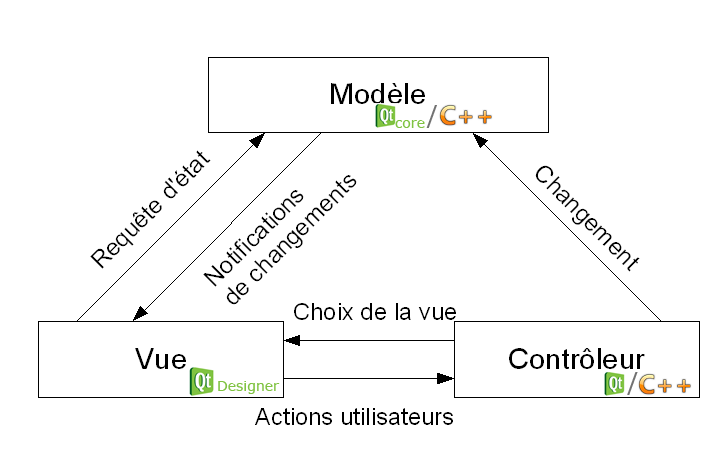
\includegraphics[width=1\textwidth]{mvc.png}
  	\caption{Architecture MVC avec Qt}
    \label{fig:diagramme-mvc}
\end{figure}


\section{Tests du logiciel}

\subsection{Tests unitaires}

Nous écrirons ces tests au fur et à mesure du développement de notre logiciel, si possible avant même d'écrire le code à tester.
Toute unité de code \footnote{Dans notre contexte, une unité de code sera vraisemblablement une méthode comme nous ferons de la programmation orientée objet.} non-triviale pouvant être testée avec des tests unitaires devra l'être.
L'objectif est ici d'assurer la plus grande couverture de code pour éviter toute régression.


\subsection{Tests empiriques}

\subsubsection{Estimation du modèle GARCH}

L'estimation du modèle GARCH fait partie de nos algorithmes un peu délicat, notamment pour le tester.
Nous utiliserons donc un test un peu particulier.
Nous générerons tout d'abord, à l'aide de R, un ensemble de données à partir d'un modèle GARCH théorique.
Nous aurons ainsi l'assurance que ces données suivent notre modèle GARCH.
Nous pourrons donc ensuite estimer un modèle GARCH qui sera comparé au modèle théorique.

\subsubsection{Calcul de la Value-at-Risk à partir d'un modèle GARCH}

Le second algorithme délicat à tester est celui calculant la Value-at-Risk à partir d'une modélisation GARCH.
De même, pour tester ce dernier nous effectuerons du backtesting avec des données générées depuis un modèle GARCH théorique.
L'algorithme de backtesting \footnote{Voir \ref{backtesting-modele-garch} pour des explications sur le fonctionnement de l'algorithme.} devrait donc retourner une valeur comprise dans un intervalle connu. 
En effet, cet intervalle est celui d'un théorème central limite avec pour paramètre le risque pris lors du calcul de la Value-at-Risk.

Ce deuxième test empirique dépend à la fois du calcul du modèle GARCH et de l'algorithme de Backtesting. Pour cette raison nous avons choisi de tester le premier calcul indépendamment. Le second calcul est relativement simple et pourra être l'objet d'un test unitaire \footnote{En passant en paramètre une classe anonyme dérivée de \textit{VarAlgorithm} dont nous définirons la valeur de retour.}.


\subsection{Tests fonctionnels}

Les tests fonctionnels permettront de valider chacun des cas d'utilisation classique de notre logiciel (voir le diagramme de cas d'utilisation en figure \ref{fig:usecase}).
Contrairement aux tests unitaires nous commencerons à les écrire vers la fin du projet, une fois que nous aurons suffisamment de modules opérationnels.

\subsection{Tests de l'interface graphique}

Les tests de l'interface graphique ne seront pas automatisés.
Cette opération serait trop longue à effectuer.
De plus, elle a peu d'intérêt d'un point de vue régression puisque l'interface graphique ne sera pas entièrement fonctionnelle avant la fin du projet.
Enfin cette dernière sera amenée à changer suite aux retours du client.
Avec des tests automatisés, toute modification de l'interface obligerait à modifier les tests.

Nous testerons donc cette partie manuellement au fur et à mesure de son développement et entièrement à la toute fin du projet.


\chapter*{Conclusion}

Dans ce document, nous avons commencé par rappeler les fonctionnalités du logiciel définies lors de la phase de spécification à l'aide de  diagrammes de cas d'utilisation.
Parmi celles-ci, la gestion de portefeuilles, le calcul de la Value-at-Risk ainsi que la génération de rapports occupent une place centrale.
Nous avons également présenté l'architecture générale du programme soulignant en particulier l'utilisation du module externe R pour les calculs avancées.

Nous avons ensuite détaillé la modélisation de la base de données nécessaire au stockage des informations importées ou générées afin que l'utilisateur retrouve d'une utilisation à l'autre ses portefeuilles et les rapports associés.
Nous avons poursuivi avec la présentation de notre modélisation à l'aide de diagrammes de classes ainsi que que quelques diagrammes de séquence afin de préciser les interactions les plus complexes entre les objets.
En particulier, le calcul de la Value-at-Risk basée sur un modèle GARCH ou encore le backtesting ont bénéficié de cette dernière modélisation.
Enfin nous avons abordé la modélisation de notre interface graphique ainsi que l'organisation de nos tests.

Lors de cette phase de conception nous avons été confrontés à un certain nombre de problèmes techniques auxquels nous avons dû répondre.
Ce travail est nécessaire pour la phase suivante.
En effet, nous allons maintenant pouvoir commencer le développement de notre logiciel.
Grâce à cette étape préliminaire nous allons avancer plus rapidement et sereinement; nous avons maintenant une vue précise du travail à effectuer.


\bibliographystyle{unsrt}
\bibliography{biblio}


\end{document}